\documentclass[a4paper, 10pt]{article}
\usepackage{comment} % enables the use of multi-line comments (\ifx \fi) 
\usepackage{lipsum} %This package just generates Lorem Ipsum filler text. 
\usepackage{fullpage} % changes the margin
\usepackage{graphicx}
\usepackage{xcolor}

\begin{document}
%Header-Make sure you update this information!!!!
\noindent
\large\textbf{Middleware Project - IoT} \hfill \textbf{Marco Bacis} 873199 \\
Prof. Mottola \hfill \textbf{Daniele Cattaneo} 874757 \\
Prof. Guinea

\section*{Problem Statement}

The goal of the project is to develop an IPv6-based presence detection system using MQTT, in which every person is equipped with a wireless sensor, and every room has a static wireless device working as IPv6 border-router.
The mobile device detects the user movements and, when the user is stationary, sends messages to a MQTT broker with the client id, in a different channel for each room.
The device should do everything possible to minimize energy consumption while the user is moving.
Finally, the client application must contain parameters for the movement threshold (T) and for the acceleration reading period while the used is motionless (G), along with all the other relevant constants, in the project-conf.h file.

\section*{Implementation}

\subsection*{Sensor Finite State Machine}

\begin{figure}[h]
\centering
    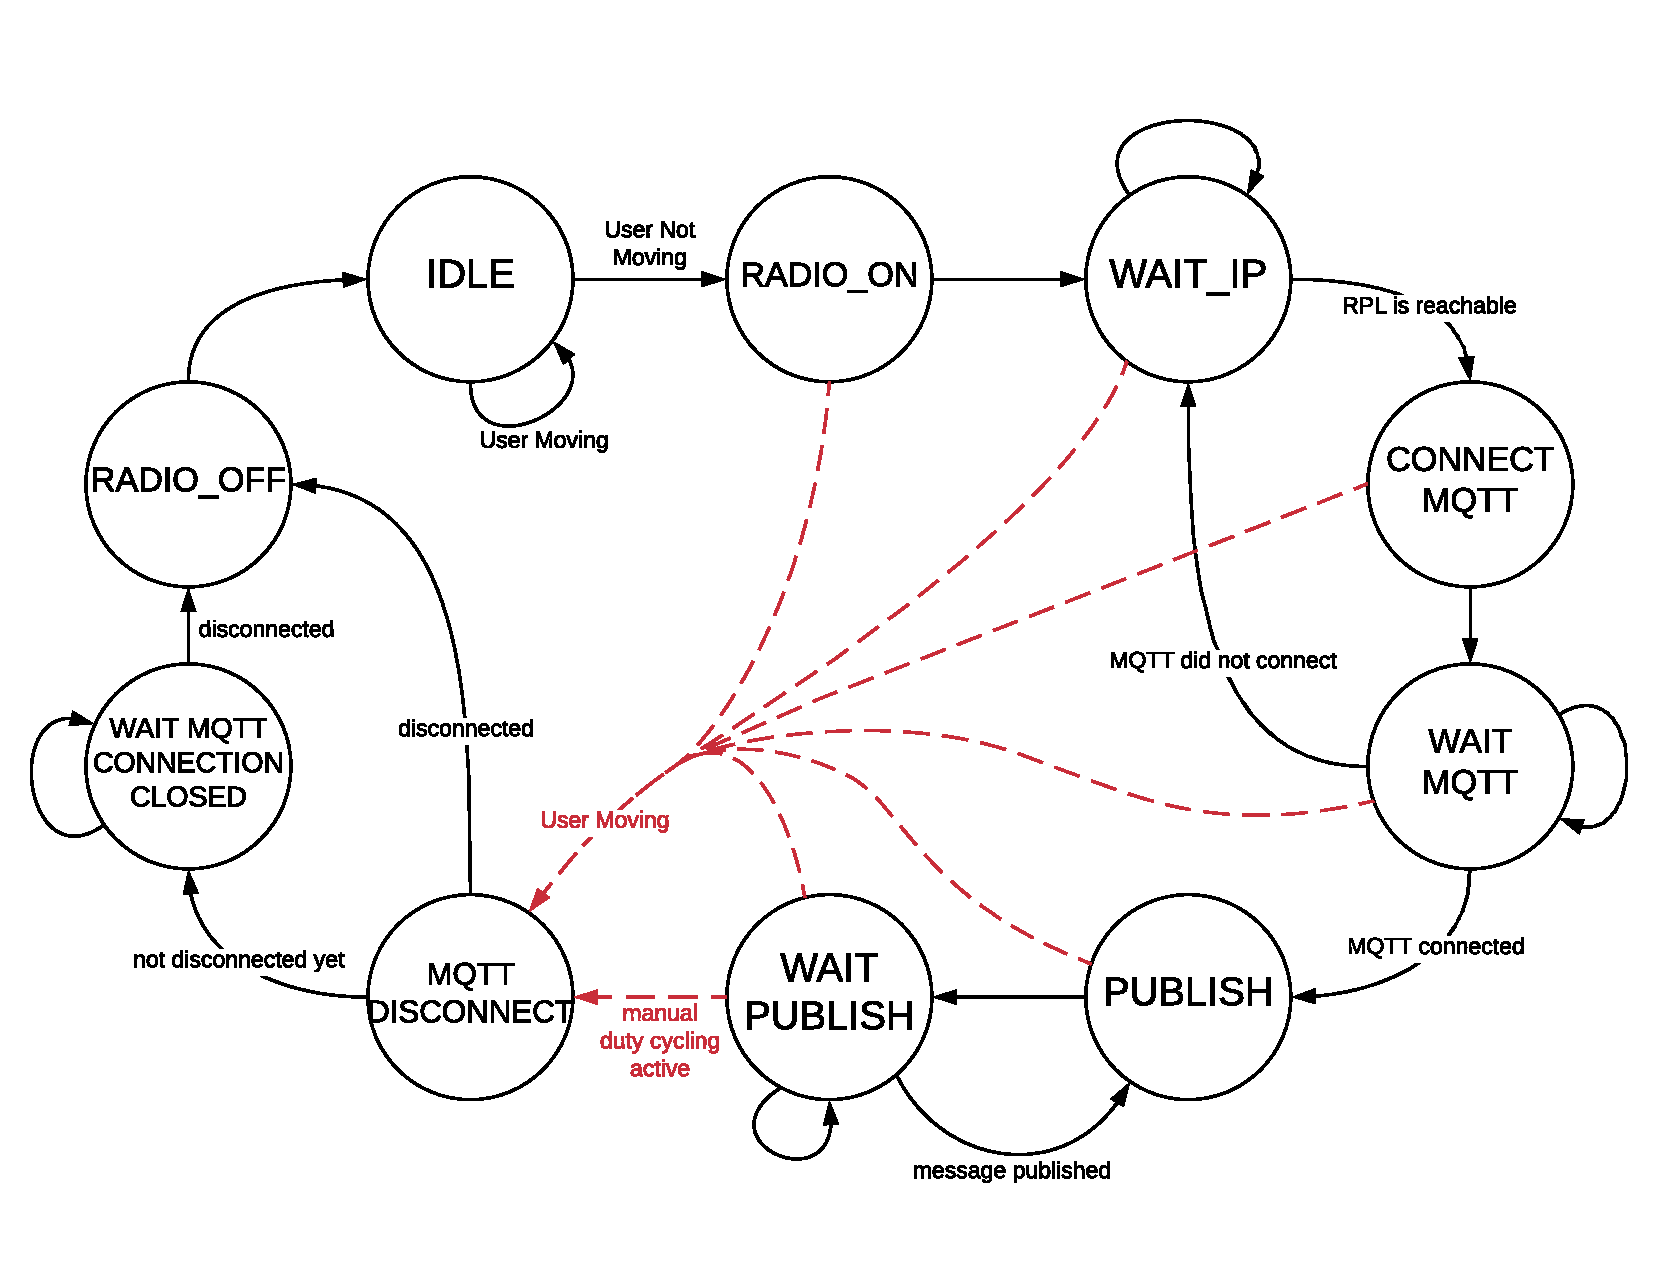
\includegraphics[width=\linewidth]{images/fsm.pdf}
    \caption{Sensors Finite State Machine responsible for the radio/mqtt connection and publishing}
    \label{fig:sensor_fsm}
\end{figure}

The main sensor thread (client\_process) integrates a Finite State Machine (FSM) to manage the mqtt connection based on the reachability of a IP network and the user movements.
The FSM process is event-driven (being a contiki protothread), but also has a default timer of one second when waiting for long events (such as connections and disconnections).
The FSM can be seen in Figure~\ref{fig:sensor_fsm}, which highlights the states and relevant transitions.
The source and sink state is IDLE, in which the sensor doesn't perform any action apart from waiting for the user to stop moving.

When the user stops moving, the connection is initialized by turning the radio on and waiting for an IP and MQTT connection to be estabilished. 
After that, a json message is published every K seconds on the root border-router id (which acts as room id).
The message format is \{client\_id, seq\_number, last\_accel, current\_rssi, current\_dbm\_power, uptime\}.

Two global events are also handled. The first is when the user starts moving (detected by the movement monitor process), while the other is connection lost (either MQTT or RPL not reachable). In both cases, the state is changed to \emph{MQTT\_DISCONNECT} and the disconnection phase is performed, waiting for the next opportunity to connect.

\subsection*{Parameters Estimation}

\begin{figure}[h]
\centering
    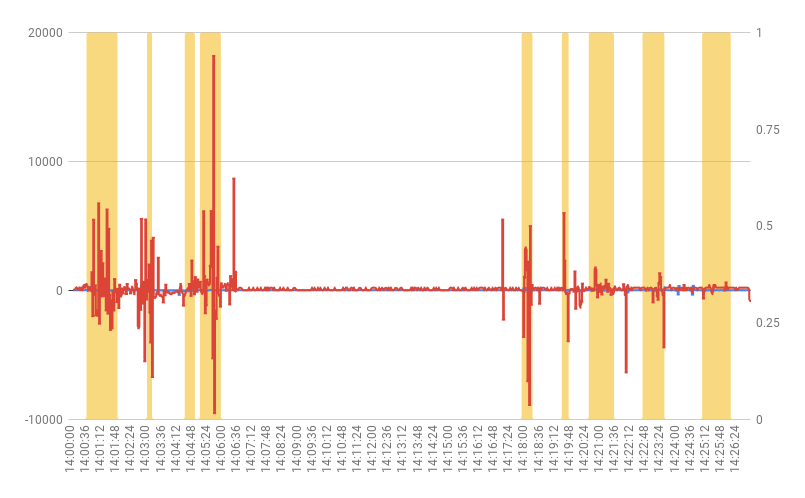
\includegraphics[width=0.7\linewidth]{images/accel_chart.png}
    \caption{Gathered movement data (module - gravity) with movement periods highlighted}
    \label{fig:accel_data}
\end{figure}

Two parameters were estimated: T (movement threshold) and G (movement read timeout while not moving).

For both parameters, real data were collected using the sensortag board, and analyzed in order to get a fair estimate.
The data were collected while a user moved in his house with the sensortag attached doing menial tasks.
From the X, Y and Z acceleration readings other parameters (such as euler angles and acceleration diffs) were computed to see when the user was moving.
The accelerator data and the detected movement is shown in Figure~\ref{fig:accel_data}.

The movement threshold T is applied to the absolute value of the acceleration module minus the gravity acceleration module, so it was estimated by trying to match the estimated movements with the real ones. We estimated $T = 1000$ roughly. Also, a second threshold T\_DMOD is applied to the difference between the current and last modules, and has been set to half the general treshold. 

The reading timeout G is a environment and use-case dependent factor, as it depends on the place in which the system is deployed and which activities the users are usually doing.
Different measures can be used to estimate its value.
The measure of G impacts on the resolution of the system (not counting disconnections when moving too far from the router), so it must be a lower bound based on some experimental data gathered from the environment.
In our case, we used a \emph{smooth} representation of the acceleration data to obtain the movements (without counting micromovements in the same room).
The average movement lasted 42 seconds with a $23,29$ standard deviation, a minimum time of 12 seconds and maximum of 74 seconds.
As a tradeoff between resolution and energy consumption we decided to estimate G as $average - standard deviation$ from the test data, meaning $G = 19$ seconds.
In this way, G lasts less than $84,1$\% of the movement periods, and at least one acceleration measure is done in longer periods.

\subsection*{Energy Consumption minimization}
In order to reduce the energy consumption of the device, two features were added to the client code, one for acceleration readings and the other for the network connection.

As for the data movement reading, the movement sesor (MPU 9250) is activated only when necessary (only while reading). 

The network connections impacts heavily on the client energy consumption. To reduce this, two options can be configured in the client code: TSCH or manual CSMA duty cycling.

With TSCH, the duty cycling mechanism is handled transparently underneath RPL, meaning that the radio is controlled with a coarse grained approach (user moving or not moving implies client connected or not).

Instead, when manual duty cycling is enabled in CSMA mode, the radio is kept on only for the duration of time needed to  connect to the MQTT broker and send a single message, then it is turned  off immediately.
Moreover, to avoid excessive power consumption for small values of K, when manual duty cycling is on, K is effectively increased by the amount of  time needed to connect to the RPL network after the radio is turned on.

Table~\ref{table:energest} shows some test results for the two modes.
Each test was runned on the board for 10 minutes, by forcing the sensor to consider a moving or motionless user.
It can be seen that manual duty cycling over CSMA (DutyCycling) has the lowest possible power draw while the user is moving, and is low also while motionless, as it drastically reduces the CPU activity.
On the other hand, TSCH has a lower energy consumption while motionless, but it keeps the CPU active for longer periods, to check the radio state transparently and not manually.


\begin{table}[!htb]
\begin{tabular}{ll|ccc|cc|c}
& & \multicolumn{3}{c|}{ \textbf{CPU Mode (s)} } & \multicolumn{2}{c|}{ \textbf{Radio (s)} } & \\
\textbf{MAC} & \textbf{Action} & \textbf{Active} & \textbf{Sleep} & \textbf{Deep Sleep} & \textbf{Listening} & \textbf{Transmit} & \textbf{Energy (J)} \\
CSMA & Motionless & 1 & 2 & 596 & 0 & 0 & 0.05 \\
CSMA & Moving & 13 & 581 & 5 & 592 & 2 & 11.59 \\
CSMA & DutyCycling & 13 & 273 & 312 & 280 & 3 & 5.58 \\
TSCH & Moving & 174 & 24 & 401 & 163 & 0 & 8.39 \\
TSCH & Standing & 157 & 28 & 414 & 53 & 3 & 2.43 \\
TSCH & StandNoLed & 209 & 22 & 367 & 107 & 2 & 3.81 \\
\end{tabular}
\caption{Energest test data}
\label{table:energest}
\end{table}

%\section*{Attachments}
%Make sure to change these
%Lab Notes, HelloWorld.ic, FooBar.ic
%\fi %comment me out


\end{document}
